% !TeX program = pdflatex
% LISA Challenge 2026 --- single team paper covering Task 1A, Task 1B and Task 2.
% Springer LNCS, target 8--10 pages body + references.
\documentclass[runningheads]{llncs}

% ---------------------------------------------------------------------------
% Packages
% ---------------------------------------------------------------------------
\usepackage[T1]{fontenc}
\usepackage{graphicx}
\usepackage{booktabs}
\usepackage{amsmath}
\usepackage{amssymb}
\usepackage{multirow}
\usepackage{placeins}
\usepackage{xcolor}
\usepackage{colortbl}
\usepackage[hidelinks]{hyperref}
\setlength{\emergencystretch}{3em}
\graphicspath{{figures/}{./}}

% Tighten float spacing to pack tables/figures across the page limit
\setlength{\textfloatsep}{8pt plus 2pt minus 2pt}
\setlength{\floatsep}{8pt plus 2pt minus 2pt}
\setlength{\intextsep}{8pt plus 2pt minus 2pt}
\renewcommand{\textfraction}{0.05}
\renewcommand{\topfraction}{0.92}
\renewcommand{\bottomfraction}{0.92}
\renewcommand{\floatpagefraction}{0.85}

% ---------------------------------------------------------------------------
% Table group colours (from the Task 2 paper)
% ---------------------------------------------------------------------------
\definecolor{clrGroupA}{HTML}{EFF3FF}
\definecolor{clrGroupB}{HTML}{F0FFF0}
\definecolor{clrGroupC}{HTML}{FFF0F5}
\definecolor{clrGroupD}{HTML}{FFF5EB}

\begin{document}

% ===========================================================================
\title{Rigor over Novelty in Ultra-Low-Field Pediatric Brain MRI:
Quality Control and Subcortical Segmentation for the LISA Challenge 2026\\
\large Synapse Project ID: syn75277286}
\titlerunning{Rigor over Novelty in ULF Pediatric Brain MRI}

\author{Anonymous Author(s)}
\authorrunning{Anonymous}

\institute{Anonymous Institution}

\maketitle

% ===========================================================================
\begin{abstract}
Ultra-low-field (ULF) MRI at 0.064\,T extends neuroimaging to resource-limited
and pediatric settings, but its low signal-to-noise ratio, weak boundary
contrast and coarse resolution challenge automated analysis. We report a single
team submission to three tracks of the LISA Challenge~2026 and organise it around
one methodological thesis: at this field strength the reliable gains come from
rigour --- leakage-free evaluation, faithful validation, honest curation --- and
not from architectural novelty. For \textbf{Task~1A} (multi-label artifact
grading over seven classes at three ordinal severity levels) we model the target
in its native ordinal form with two cumulative heads, an ordinal focal loss and a
monotonicity penalty, and evaluate a ten-model cross-validated ensemble strictly
on out-of-fold predictions, reaching a challenge-metric micro-accuracy of
\textbf{0.839}. For \textbf{Task~1B} (low-field image-quality enhancement) we
show through a controlled study that a carefully normalised native-resolution
pass-through is a strong, overfitting-free baseline that our four learned
enhancers fail to beat; we diagnose three concrete causes --- self-inflicted
preprocessing damage, a cross-field-strength registration ceiling near
$0.5$--$0.6$ correlation that makes supervision hallucinate, and a
metric-overfitting (Goodhart) effect in checkpoint selection. For
\textbf{Task~2} (3D segmentation of nine scored subcortical structures) a
residual-encoder nnU-Net trained on the full cohort with stock components attains
a mean Dice of \textbf{0.785}, and an inference study shows that
structure-specific connected-component post-processing is locally optimal while
uniform filtering deletes real anatomy. Across all three tasks a well-configured,
honestly validated pipeline is competitive, and we argue such baselines should be
reported before novelty is claimed.
\keywords{Ultra-low-field MRI \and Pediatric neuroimaging \and Image quality
assessment \and Artifact grading \and Image enhancement \and Subcortical
segmentation \and nnU-Net}
\end{abstract}

% ===========================================================================
\FloatBarrier
\section{Introduction}
\label{sec:intro}

Portable MRI scanners operating at or below 0.1\,T have moved from laboratory
curiosity to clinically deployed imaging~\cite{marques2019low,sheth2021portable}.
The Hyperfine Swoop, at 0.064\,T, needs no radio-frequency shielding and runs
from a standard wall outlet, making point-of-care and pediatric imaging feasible
where a conventional 1.5--3\,T system is unaffordable --- precisely for the
populations that most lack access to high-field MRI, and in which early imaging of
brain development would be most valuable~\cite{arnold2023low,sarracanie2020}.
The clinical price of this accessibility is image quality: at 0.064\,T the
signal-to-noise ratio is roughly two orders of magnitude below a clinical
scanner, contrast between adjacent gray-matter structures is weak, and the
recoverable resolution is coarse relative to the structures of interest.

The LISA Challenge~2026 targets this regime with a quality-control (QC) track and
a segmentation track. \textbf{Task~1A} asks for automated quality assessment:
grading seven artifact classes (Noise, Zipper, Positioning, Banding, Motion,
Contrast, Distortion) at three ordinal severity levels ($0$~=~none, $1$~=~mild,
$2$~=~severe) per acquisition plane. \textbf{Task~1B} asks for image-quality
\emph{enhancement}: mapping a ULF stack toward a high-field isotropic reference
under a battery of distributional and no-reference metrics. \textbf{Task~2} asks
for 3D segmentation of subcortical gray matter, scored over nine structures.

This paper is a single account of one team's participation across all three
tasks, unified by a deliberate methodological posture. Low-field pediatric data
are scarce, noisy and easily over-fit; in that setting we found that the
dependable improvements came not from bespoke architectures but from getting the
evaluation, validation and curation right. Concretely, our contributions are:
\begin{enumerate}
  \item \textbf{(Task~1A)} An ordinal, cumulative-head formulation that matches
        the challenge's native $\{0,1,2\}$ metric, trained as a two-backbone,
        five-fold deep ensemble and evaluated with a strictly leakage-free
        out-of-fold (OOF) protocol, reaching micro-accuracy 0.839.
  \item \textbf{(Task~1B)} A controlled demonstration that a well-normalised
        native pass-through is a strong, overfitting-free baseline, together with
        a diagnosis of the registration ceiling, preprocessing damage and
        metric-overfitting effects that prevented four learned enhancers from
        beating it.
  \item \textbf{(Task~2)} A no-frills residual-encoder nnU-Net that reaches mean
        Dice 0.785 over the nine scored labels, with an inference-tuning study
        whose clear negative result is that uniform connected-component
        post-processing degrades surface accuracy relative to nnU-Net's
        structure-specific scheme.
\end{enumerate}

% ===========================================================================
\FloatBarrier
\section{Methods}
\label{sec:methods}

\subsection{Task~1A --- Ordinal Artifact Grading}
\label{sec:m1a}

\paragraph{Data and preprocessing.}
The Task~1A training set comprises 532 per-plane images from 244 acquisitions on
the Hyperfine Swoop, each annotated with a $\{0,1,2\}$ severity for all seven
artifact classes. Labels are assigned \emph{per plane}: the axial, coronal and
sagittal planes of a subject can carry different grades, since each is an
independent acquisition. The severity distribution is severely imbalanced
(Table~\ref{tab:perclass}): Banding has only 21 positive planes (4\%) against
Contrast's 197 (37\%), and about 47\% of planes carry two or more simultaneous
artifacts, motivating a multi-label treatment. From each NIfTI stack we form a
three-channel image from the slices at the 25th, 50th and 75th percentile
positions along the through-plane axis, so every channel carries independent
volumetric evidence. Each channel is windowed to its 1st--99th intensity
percentiles and rescaled to $[0,1]$, making the pipeline invariant to the mixed
integer/float encodings in the data; images are resized to $256\times256$ and
normalised with ImageNet statistics. Augmentation is purely geometric
(flips, $\pm15^\circ$ rotation, small translation and scaling); intensity-altering
augmentations are excluded because MRI intensity statistics are diagnostic for
Noise, Contrast and Banding.

\paragraph{Ordinal architecture and loss.}
The challenge ranking is the flattened multi-class micro-average over the
severity grid: with $C$ classes and $N$ images, every one of the $C\times N$
cells contributes a single $\{0,1,2\}$ prediction, and for a flattened
multi-class problem micro precision, recall, $F_1$ and $F_2$ all equal accuracy,
so the composite score reduces exactly to \emph{micro-accuracy}, which we
optimise directly. We model each class ordinally rather than binarising severity.
Each backbone (feature dimension $d$) feeds a shared trunk
$\text{Dropout}(0.4)\!\to\!\mathrm{FC}(d\!\to\!512)\!\to\!\mathrm{ReLU}
\!\to\!\mathrm{BN}$ and two cumulative heads that emit, per class, the logits for
$P(\text{severity}\ge 1)$ and $P(\text{severity}\ge 2)$. The grade is recovered as
\[
  \hat{y}_c =
  \begin{cases}
    2 & \text{if } P_c(\ge 2)\ge t^{(2)}_c,\\
    1 & \text{else if } P_c(\ge 1)\ge t^{(1)}_c,\\
    0 & \text{otherwise,}
  \end{cases}
\]
and training minimises an ordinal focal loss over both heads,
\[
  \mathcal{L} = \mathcal{L}^{\mathrm{focal}}_{\ge 1}
              + w_2\,\mathcal{L}^{\mathrm{focal}}_{\ge 2}
              + w_{\mathrm{mono}}\,
                \mathbb{E}\big[\,\mathrm{ReLU}\!\big(P(\ge 2)-P(\ge 1)\big)\big],
\]
with focal exponent $\gamma=2$~\cite{lin2017focal}, a heavier weight $w_2=4$ on
the rarer severe head, and a monotonicity penalty ($w_{\mathrm{mono}}=0.5$)
enforcing $P(\ge 2)\le P(\ge 1)$~\cite{frank2001simple}. A severity-stratified
sampler injects at least one $\ge 1$ and one $\ge 2$ anchor per class into every
mini-batch, guaranteeing gradient signal for rare classes such as Banding.

\paragraph{Training, ensemble and calibration.}
Each backbone is fully fine-tuned with AdamW (learning rate $10^{-4}$, weight
decay $5\!\times\!10^{-2}$), a 5-epoch warm-up and cosine schedule, batch size 16,
gradient clipping at 0.5, up to 100 epochs with early stopping (patience 20). We
train EfficientNet-B4 and ConvNeXt-Small under a five-fold
\emph{StratifiedGroupKFold} split grouped by acquisition, so no subject leaks
across folds. The final predictor averages the sigmoid outputs of all ten models
(2 backbones $\times$ 5 folds), each with eight-way dihedral test-time
augmentation~\cite{lakshminarayanan2017simple}. Per-class thresholds
$t^{(1)}_c,t^{(2)}_c$ are searched on OOF predictions to maximise micro-accuracy,
and a calibrated threshold is accepted only if it improves the score in at least
four of the five folds; otherwise the class keeps the default $0.5$. For the
shifted testing phase we additionally define a label-free \emph{transport} rule:
for each class the test threshold is set to the quantile of the test-probability
distribution that reproduces the positive fraction observed at the calibrated OOF
threshold, neutralising a monotone covariate shift without test labels.

\subsection{Task~1B --- Low-Field Image-Quality Enhancement}
\label{sec:m1b}

\paragraph{Data and task.}
Each subject provides one or more anisotropic low-field stacks (axial, coronal,
sagittal; $1.5$\,mm in-plane, $5$\,mm through-plane); when available a high-field
isotropic reference (CISO, $1$\,mm) is provided for supervision and scoring, and
is \emph{not} voxel-aligned to the low-field stacks. Enhanced volumes must retain
the exact input geometry and are scored against CISO with a mixture of
distributional metrics (Fr\'echet Inception Distance, FID~\cite{heusel2017fid};
Fr\'echet Radiomics Distance, FRD), a learned perceptual distance
(LPIPS~\cite{zhang2018lpips}), a full-reference fidelity metric (PSNR), and two
no-reference perceptual metrics (BRISQUE~\cite{mittal2012brisque} and
CLIP-IQA~\cite{wang2023clipiqa}). These metrics reward conflicting behaviours, so
a method can improve one while destroying another. All processing operates on 2-D
slices along the thin axis; each slice is normalised to $[0,1]$ by its 1st--99th
intensity percentile, identically across every method and every metric
computation to avoid normalisation-induced confounds.

\paragraph{Enhancement strategies.}
We evaluated a progression of learned methods against a minimal control; all
learned models share a Residual U-Net backbone~\cite{ronneberger2015unet}
($\approx7.6$\,M parameters, four encoder levels, instance normalisation, global
residual) on a $160\times160$ native canvas.
\emph{(M1) Physics-augmented residual denoiser}: a ResUNet trained on the clean
partition with synthetic degradation (Rician noise plus $k$-space motion
ghosting) and a $0.6\,\mathcal{L}_1+0.4\,(1-\mathrm{SSIM})$ objective; on real
input its residual is near-zero.
\emph{(M2) Resampled-target supervised translator}: a ResUNet mapping low-field
slices to CISO brought onto the low-field grid by array resizing (no
registration).
\emph{(M3) Unpaired adversarial translator}: an LSGAN~\cite{mao2017lsgan} with a
PatchGAN discriminator pushing outputs toward the CISO distribution, anchored by
an $\mathcal{L}_1{+}$SSIM term; checkpoints selected by the local FID proxy.
\emph{(M4) Registered supervised translator with perceptual loss}: CISO is
registered to each stack with a rigid multi-resolution Mattes mutual-information
transform~\cite{mattes2003}, then a ResUNet is trained toward the registered
target with $0.5\,\mathcal{L}_1+0.3\,(1-\mathrm{SSIM})+0.1\,\mathcal{L}_
\mathrm{VGG}$~\cite{johnson2016perceptual}.
\emph{(C) Native normalisation pass-through}: \emph{no} learned enhancement ---
each slice is percentile-normalised at native resolution and written back with
the original geometry, no resize and no 8-bit quantisation, isolating
preprocessing hygiene from learned enhancement.

\paragraph{Faithful local validation.}
The challenge grants few submissions, so we reproduce the scorer's no-reference
metrics (BRISQUE, CLIP-IQA) and an InceptionV3-FID against the CISO distribution
locally with the \texttt{piq} library. Absolute values differ from the server,
but two properties hold and are what we rely on: local FID \emph{orders}
non-adversarial submissions consistently with the server, and the BRISQUE change
relative to the input is directionally faithful. For model selection we require a
candidate to beat the control on held-out FID \emph{without} regressing
BRISQUE --- an explicit guard against metric overfitting.

\subsection{Task~2 --- Subcortical Segmentation}
\label{sec:m2}

\paragraph{Data and label protocol.}
The training set comprises 79 cases, each a single CISO-reconstructed volume with
a manual ground-truth segmentation of eleven structures: background, left/right
hippocampus, left/right lateral ventricle, left/right caudate, left/right
lentiform nucleus (putamen and globus pallidus merged), left/right thalamus, and
the corpus callosum. A scoring detail shapes every design decision: the two
ventricle labels are \emph{not} scored. The ranking is computed over the nine
remaining labels, aggregating five metrics --- $1-$DSC, HD, HD95, ASSD (mm) and
relative volume error (RVE, \%) --- with lower better and bilateral sides
averaged~\cite{maierhein2024metrics}. No external data were used.

\paragraph{Quality control and curation.}
Annotation quality was screened before training. For each structure we
standardised per-case volumes across the cohort and flagged any case with a
per-structure volume $z$-score above three in magnitude. Six of 79 cases were
flagged and inspected slice by slice; in every instance the extreme volume
tracked real anatomy (enlarged ventricles, a genuinely large or small
hippocampus) with boundaries following the image, so we excluded none. Retaining
all 79 is deliberate: at this cohort size the cost of discarding valid rare
anatomy outweighs the risk of a few atypical volumes, a markedly more
conservative posture than pipelines that drop a large fraction of the cohort on
automated criteria.

\paragraph{Network, training and inference.}
We use nnU-Net~v2~\cite{isensee2021nnunet} with the residual-encoder preset
ResEncUNetM~\cite{isensee2024revisited}, configuration \texttt{3d\_fullres} and
the default trainer --- a ResidualEncoderUNet with six stages and
$[32,64,128,256,320,320]$ features, sized for a single 16\,GB GPU. The
fingerprint step resampled volumes to $1\times1\times1$\,mm and set a patch of
$112\times160\times128$ with batch size~2. Training follows the stock schedule
(1000 epochs per fold, Dice-plus-cross-entropy with deep supervision, SGD with
Nesterov momentum, polynomial decay, standard spatial and intensity
augmentation); no custom loss, sampler or augmentation was introduced. All five
folds completed on an NVIDIA RTX~4070~Ti~SUPER (16\,GB). Final predictions come
from the five-fold ensemble with mirroring test-time augmentation. Inference is a
sliding window whose \texttt{step\_size} we treat as tunable
(Section~\ref{sec:r2}). For post-processing, nnU-Net's automatic step selected
largest-connected-component (LCC) filtering for labels $\{3,4,7\}$ (the two
ventricles and left lentiform) and left the rest untouched; we adopt this
structure-specific scheme and test it against uniform and milder alternatives. A
second recipe merging each left/right pair into a bilateral class (six classes)
with mirroring augmentation was only partially trained (one fold) and is reported
as future work, not as an evaluated alternative.

% ===========================================================================
\FloatBarrier
\section{Results}
\label{sec:results}

\subsection{Task~1A --- Ordinal Artifact Grading}
\label{sec:r1a}

All Task~1A results are computed on leakage-free five-fold OOF predictions over
the 532 training planes; no test-set or leaderboard information is used.
Table~\ref{tab:ensemble} shows the two backbones are individually comparable
($\approx0.827$ calibrated) and that ensembling with TTA lifts OOF micro-accuracy
to 0.839, with anti-overfit calibration adding $+0.011$ over the naive $0.5$
operating point.

\begin{table}[htbp]
\caption{Task~1A ensemble ablation on OOF predictions (micro-accuracy over the
flattened $\{0,1,2\}$ grid). Calibration is the anti-overfit per-class threshold
search of Section~\ref{sec:m1a}.}
\label{tab:ensemble}
\centering
\setlength{\tabcolsep}{8pt}
\begin{tabular}{lcc}
\toprule
Configuration & @\,$0.5/0.5$ & Calibrated \\
\midrule
EfficientNet-B4 (5 folds)      & 0.820 & 0.827 \\
ConvNeXt-Small (5 folds)       & 0.824 & 0.827 \\
Ensemble (10 models) + TTA     & \textbf{0.828} & \textbf{0.839} \\
\bottomrule
\end{tabular}
\end{table}

Table~\ref{tab:perclass} breaks the score down by class. Rare classes dominated
by true negatives (Banding, Noise, Positioning) achieve the highest three-way
accuracy, whereas high-prevalence classes (Motion, Contrast, Distortion) are
hardest. The quadratic weighted $\kappa$ (QWK), which penalises grading errors by
ordinal distance, is highest for Noise (0.82) and Motion (0.71) and lowest for
Positioning (0.46) and Distortion (0.46) --- the artifacts with the least
stereotyped spatial signature, and the natural targets for future work.

\begin{table}[htbp]
\caption{Task~1A per-class OOF performance of the ensemble at calibrated
thresholds. $n_1,n_2$ are mild/severe plane counts; Acc.\ is three-way accuracy;
QWK is quadratic weighted $\kappa$ over $\{0,1,2\}$.}
\label{tab:perclass}
\centering
\setlength{\tabcolsep}{6pt}
\begin{tabular}{lccccc}
\toprule
Class & $n_1$ & $n_2$ & Acc. & QWK & $(t^{(1)}, t^{(2)})$ \\
\midrule
Banding     &   9 & 12 & 0.970 & 0.671 & (0.55, 0.25) \\
Noise       &  42 & 51 & 0.908 & 0.820 & (0.65, 0.35) \\
Positioning &  45 & 25 & 0.870 & 0.455 & (0.65, 0.35) \\
Zipper      & 142 & 37 & 0.812 & 0.644 & (0.50, 0.50) \\
Motion      &  93 & 76 & 0.771 & 0.705 & (0.60, 0.25) \\
Contrast    & 166 & 31 & 0.771 & 0.608 & (0.50, 0.40) \\
Distortion  &  95 & 49 & 0.771 & 0.458 & (0.65, 0.55) \\
\midrule
\textbf{Mean} & & & \textbf{0.839} & \textbf{0.623} & --- \\
\bottomrule
\end{tabular}
\end{table}

\subsection{Task~1B --- Low-Field Enhancement}
\label{sec:r1b}

Table~\ref{tab:board} reports the official validation-leaderboard metrics.
Among our configurations the native pass-through (C) is best or tied-best on
every metric except FID, where it is within one point of the physics denoiser; it
uniquely achieves a \emph{negative} BRISQUE change and the lowest FRD. The
resampled-target translator (M2) is by far the worst, and the adversarial
translator (M3) trades a small CLIP-IQA gain for worse FID and FRD.

\begin{table}[htbp]
\caption{Task~1B official validation-leaderboard metrics. Arrows indicate the
favourable direction; $\Delta$ values are changes relative to the input low-field
image. Best value \emph{among our submissions} in bold; the top team is shown for
context only.}
\label{tab:board}
\centering
\small
\begin{tabular}{lcccccc}
\toprule
Method & FID\,$\downarrow$ & LPIPS\,$\downarrow$ & PSNR\,$\uparrow$ &
$\Delta$BRISQUE\,$\downarrow$ & $\Delta$CLIP-IQA\,$\uparrow$ & FRD\,$\downarrow$ \\
\midrule
M1 physics denoiser        & 130.35 & 0.467 & 11.80 & $+8.64$ & $+0.041$ & 9.35 \\
M2 resampled target        & 210.46 & 0.501 & 11.53 & $+27.0$ & $+0.084$ & 18.55 \\
M3 unpaired adversarial    & 136.88 & \textbf{0.461} & 11.93 & $+7.83$ & \textbf{$+0.066$} & 9.89 \\
\textbf{C native pass-through} & \textbf{131.37} & 0.465 & \textbf{11.95} &
\textbf{$-4.76$} & $-0.018$ & \textbf{7.10} \\
\midrule
Top team (context)         & 114.57 & 0.457 & 12.07 & $-0.91$ & $+0.016$ & 10.65 \\
\bottomrule
\end{tabular}
\end{table}

\paragraph{Local proxy fidelity and the Goodhart effect.}
For methods \emph{not} selected against the local metric, the local-to-server FID
ratio is stable ($\approx1.6$): the resampled target is correctly ranked far
worse than the physics baseline both locally and on the server. The adversarial
translator breaks this --- selected by local FID, it attains the best local score
of all methods ($67.3$) yet its local-to-server ratio jumps to $2.03$ and it is
worse than the baseline on the server. This is a textbook Goodhart failure:
optimising the proxy detaches it from the target, which is why our M4 selection
required held-out FID plus a BRISQUE non-regression guard.

\paragraph{No fixed operator beats the untouched image.}
On 12 held-out complete subjects the identity (native pass-through) is the FID
optimum among fixed operators: unsharp masking, gamma, CLAHE and
denoise-then-sharpen all \emph{increase} per-subject FID (from $138.7$ for
identity up to $151.7$ for aggressive unsharp) and BRISQUE, so the
percentile-normalised native image already sits at a joint optimum.

\paragraph{Registration ceiling and the failure of supervised translation.}
Table~\ref{tab:reg} evaluates three ways of bringing CISO onto a low-field grid.
Array resizing (the M2 target) yields only $0.36$ mean foreground correlation,
and affine-header resampling is worse ($0.25$). Rigid mutual-information
registration nearly doubles alignment to $0.63$, improving every subject --- yet
across the full training set the registered correlation averages only $0.45$,
because cross-field-strength contrast differences and low-field distortion cap
rigid registration. Even with correct registration, the M4 perceptual translator
fails to beat the control: \emph{every} checkpoint raises held-out FID from
$138.7$ to $164$--$173$ and $\Delta$BRISQUE to $+24$ or more, flat across epochs,
so at $\approx0.5$ alignment the model is forced to hallucinate high-field texture
in slightly wrong locations. Our selection guard correctly rejected all M4
checkpoints.

\begin{table}[htbp]
\caption{Task~1B low-field-to-CISO alignment (mean foreground correlation).
Rigid mutual-information registration nearly doubles alignment over array
resizing, but tops out near $0.5$--$0.6$.}
\label{tab:reg}
\centering
\small
\begin{tabular}{lc}
\toprule
Alignment method & Correlation \\
\midrule
Array resize (the M2 target)        & 0.363 \\
Affine-header resample              & 0.251 \\
Rigid + mutual information (M4)     & \textbf{0.632} \\
\bottomrule
\end{tabular}
\end{table}

\paragraph{Preprocessing hygiene.}
The pass-through control isolates the cost of common preprocessing choices. Our
M1 submission applied resize-to-$256$ and 8-bit quantisation before scoring;
replacing this with native resolution and float output moved the server BRISQUE
change from $+8.6$ to $-4.8$ at essentially unchanged FID. A substantial part of
the ``enhancement'' problem is therefore simply avoiding self-inflicted
degradation.

\subsection{Task~2 --- Subcortical Segmentation}
\label{sec:r2}

All Task~2 numbers are computed against manual ground truth on the five-fold OOF
ensemble over all 79 cases, reported over the nine scored labels. Reducing the
sliding-window \texttt{step\_size} from the default $0.5$ to $0.3$ on a held-out
subset improved mean DSC by $+0.0042$, HD95 by $-0.004$\,mm and ASSD by
$-0.012$\,mm, with no case regressing; as the only cost is inference time we
adopted $0.3$.

A six-way post-processing ablation on the same ensemble makes the inference-tuning
point sharply. The adopted structure-specific scheme (nnU-Net's automatic LCC on
labels $\{3,4,7\}$) gives the best DSC (0.7849), HD95 (2.483\,mm) and ASSD
(0.978\,mm). Its story is clearest against a uniform policy: extending LCC to all
eleven labels barely moves DSC ($0.7849\!\to\!0.7805$) but inflates ASSD from
0.978 to 1.228\,mm --- the largest single movement, in the wrong direction. At
0.064\,T the thin tails of hippocampus and caudate are often rendered as a large
body plus small, barely-attached fragments indistinguishable from noise floaters;
uniform LCC deletes the real tail with the noise, and the surface metrics register
the amputation immediately. Three milder floater-removal variants ($<30\%$ of
largest, $<50$ voxels, and a combined rule) confirm even gentle uniform cleanup
does not pay: none beats the adopted scheme on ASSD.

Table~\ref{tab:perstruct} gives the per-structure breakdown. The hippocampus is
the bottleneck by a wide margin (both sides near Dice 0.64, worst surface
distances and volume errors), while the thalamus is the ceiling (Dice
0.876/0.875). Caudate and lentiform form a consistent middle band around
0.80--0.84. The corpus callosum is an instructive outlier: a modest Dice (0.749,
as a thin midline sheet) but the best ASSD (0.459\,mm) and RVE (7.74\,\%), since
its compact surface is localised precisely even when overlap looks unremarkable.
Fig.~\ref{fig:qual} shows the hippocampal failure mode directly.

\begin{table}[htbp]
\caption{Task~2 per-structure performance of the five-fold ensemble with the
adopted post-processing ($n=79$). The nine scored labels determine the ranking;
the two ventricle rows are shown for completeness only and do not enter the mean.}
\label{tab:perstruct}
\centering
\setlength{\tabcolsep}{5pt}
\begin{tabular}{lccccc}
\toprule
Structure & DSC\,$\uparrow$ & HD\,$\downarrow$ & HD95\,$\downarrow$ &
ASSD\,$\downarrow$ & RVE\%\,$\downarrow$ \\
\midrule
Hippocampus L & 0.627 & 5.295 & 3.653 & 1.709 & 22.95 \\
Hippocampus R & 0.654 & 4.974 & 3.515 & 1.397 & 24.03 \\
Caudate L     & 0.812 & 4.286 & 2.319 & 0.861 & 14.27 \\
Caudate R     & 0.802 & 3.766 & 2.129 & 0.818 & 11.53 \\
Lentiform L   & 0.837 & 5.181 & 2.240 & 1.024 & 13.57 \\
Lentiform R   & 0.833 & 4.174 & 2.695 & 1.101 & 16.80 \\
Thalamus L    & 0.876 & 3.813 & 2.191 & 0.763 & 11.14 \\
Thalamus R    & 0.875 & 4.072 & 2.080 & 0.666 & \phantom{0}8.79 \\
Corpus callosum & 0.749 & 4.989 & 1.520 & 0.459 & \phantom{0}7.74 \\
\midrule
\textbf{Mean (9 scored)} & \textbf{0.7849} & \textbf{4.505} & \textbf{2.483} &
  \textbf{0.978} & \textbf{14.53} \\
\midrule
\multicolumn{6}{l}{\small\itshape Non-scored (reference only)} \\
Ventricle L   & 0.790 & 4.786 & 1.913 & 0.643 & 13.55 \\
Ventricle R   & 0.772 & 5.155 & 2.153 & 0.678 & 12.70 \\
\bottomrule
\end{tabular}
\end{table}

\begin{figure}[htbp]
\centering
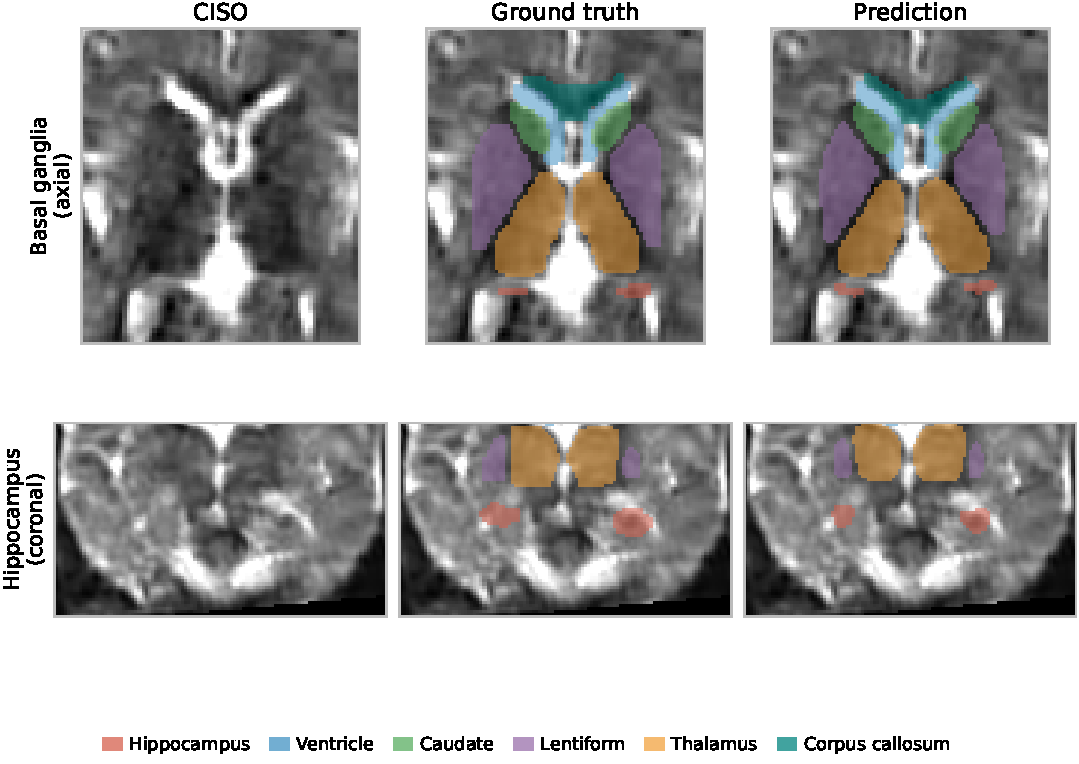
\includegraphics[width=0.7\textwidth]{figures/qual_seg.pdf}
\caption{Task~2 representative segmentation (case at the cohort-median scored
Dice, $\approx0.82$). Rows: axial through the basal ganglia, coronal through the
hippocampus. Columns: CISO volume, ground truth, prediction (ventricles drawn
but not scored). Thalamus and lentiform are recovered closely; the hippocampus
(red) is visibly under-segmented --- the thin-tail, low-contrast failure mode
behind its low Dice.}
\label{fig:qual}
\end{figure}

% ===========================================================================
\FloatBarrier
\section{Discussion}
\label{sec:discussion}

Across three tasks the same lesson recurs: at 0.064\,T a well-configured, honestly
validated pipeline is competitive, and the reliable gains come from rigour rather
than novelty.

\paragraph{Honest evaluation is a method, not an afterthought.}
In Task~1A, in-fold threshold tuning had earlier produced optimistic estimates
that did not transfer; the leakage-free OOF protocol, with a four-of-five-folds
acceptance rule for any calibrated threshold, gives an honest 0.839. In Task~2,
out-of-fold scoring over the full cohort and a zero-exclusion curation policy keep
the numbers faithful to unseen-data behaviour. Task~1B is the same discipline in
another guise: a local proxy is trustworthy for \emph{ordering} methods it did not
tune, but the adversarial translator selected against that proxy transferred
poorly, so we select on held-out data and gate candidates on a metric they were
not trained to optimise.

\paragraph{Strong baselines must be beaten, not assumed away.}
Task~1B's central finding is that a percentile-normalised native pass-through is a
joint FID/BRISQUE optimum among simple operations and beats all four learned
enhancers on the leaderboard. This is not an argument against learned enhancement
but a diagnosis of when it fails here: the input is already near-optimal for the
metrics, supervision is capped by a registration ceiling near $0.5$--$0.6$ that
makes pixel and feature losses hallucinate, and proxy-driven checkpoint selection
invites Goodhart effects. Having no learned parameters, the pass-through also
cannot overfit the validation cohort --- robustness our learned models lacked.
Task~2 carries the mirror-image lesson: connected-component filtering helps only
where a dominant component genuinely is the whole structure, and generalising it
to small filamentous gray matter deletes real anatomy (ASSD
$0.978\!\to\!1.228$\,mm), so the right move was to trust nnU-Net's per-label
selection. The residual errors are physically interpretable throughout: the
diffuse Task~1A Positioning and Distortion artifacts dominate its ordinal error,
and the Task~2 hippocampus --- small, thin, curved and weakly contrasted at
0.064\,T --- never closed its early gap, at Dice levels the physics of 0.064\,T
predicts, indicating signal-limited rather than method-limited pipelines.

\paragraph{Limitations and future work.}
Both cohorts are small and single-source, so our metrics are cross-validation
estimates on one release group, not population performance. The most promising
next steps are task-specific: better alignment for Task~1B (deformable or
contrast-invariant registration aiming for $>0.8$ correlation, to test whether
supervised enhancement can finally beat the pass-through); a boundary- or
topology-aware objective~\cite{kervadec2021boundary} and the full five-fold
symmetric-label recipe for the thin-tail hippocampal failures in Task~2; and
higher-resolution features plus validation of the label-free threshold transport
for Task~1A. All stay within the paper's premise: at 0.064\,T the gains come from
data, evaluation and inference, not from architecture.

% ===========================================================================
\begin{credits}
\subsubsection{\ackname}
Acknowledgments omitted for anonymous review.
\subsubsection{\discintname}
The authors have no competing interests to declare.
\end{credits}

% ===========================================================================
\bibliographystyle{splncs04}
\begin{thebibliography}{99}

\bibitem{marques2019low}
Marques, J.P., Simonis, F.F.J., Webb, A.G.: Low-field MRI: An MR physics
perspective. J.\ Magn.\ Reson.\ Imaging \textbf{49}(6), 1528--1542 (2019).
\url{https://doi.org/10.1002/jmri.26637}

\bibitem{sheth2021portable}
Sheth, K.N., Mazurek, M.H., Yuen, M.M., et al.: Assessment of brain injury using
portable, low-field magnetic resonance imaging at the bedside of critically ill
patients. JAMA Neurol.\ \textbf{78}(1), 41--47 (2021).
\url{https://doi.org/10.1001/jamaneurol.2020.3263}

\bibitem{arnold2023low}
Arnold, T.C., Freeman, C.W., Litt, B., Stein, J.M.: Low-field MRI: clinical
promise and challenges. J.\ Magn.\ Reson.\ Imaging \textbf{57}(1), 25--44 (2023).
\url{https://doi.org/10.1002/jmri.28408}

\bibitem{sarracanie2020}
Sarracanie, M., Salameh, N.: Low-field MRI: how low can we go? A fresh view on an
old debate. Front.\ Phys.\ \textbf{8}, 172 (2020).
\url{https://doi.org/10.3389/fphy.2020.00172}

\bibitem{lin2017focal}
Lin, T.Y., Goyal, P., Girshick, R., He, K., Doll{\'a}r, P.: Focal loss for dense
object detection. In: Proc.\ IEEE ICCV, pp.~2980--2988 (2017)

\bibitem{frank2001simple}
Frank, E., Hall, M.: A simple approach to ordinal classification. In: Machine
Learning: ECML 2001. LNCS, vol.~2167, pp.~145--156. Springer (2001)

\bibitem{lakshminarayanan2017simple}
Lakshminarayanan, B., Pritzel, A., Blundell, C.: Simple and scalable predictive
uncertainty estimation using deep ensembles. In: Advances in Neural Information
Processing Systems, vol.~30 (2017)

\bibitem{heusel2017fid}
Heusel, M., Ramsauer, H., Unterthiner, T., Nessler, B., Hochreiter, S.: GANs
trained by a two time-scale update rule converge to a local Nash equilibrium. In:
Advances in Neural Information Processing Systems, vol.~30 (2017)

\bibitem{zhang2018lpips}
Zhang, R., Isola, P., Efros, A.A., Shechtman, E., Wang, O.: The unreasonable
effectiveness of deep features as a perceptual metric. In: Proc.\ CVPR, pp.\
586--595 (2018). \url{https://doi.org/10.1109/CVPR.2018.00068}

\bibitem{mittal2012brisque}
Mittal, A., Moorthy, A.K., Bovik, A.C.: No-reference image quality assessment in
the spatial domain. IEEE Trans.\ Image Process.\ \textbf{21}(12), 4695--4708
(2012). \url{https://doi.org/10.1109/TIP.2012.2214050}

\bibitem{wang2023clipiqa}
Wang, J., Chan, K.C.K., Loy, C.C.: Exploring CLIP for assessing the look and feel
of images. In: Proc.\ AAAI, pp.~2555--2563 (2023).
\url{https://doi.org/10.1609/aaai.v37i2.25353}

\bibitem{ronneberger2015unet}
Ronneberger, O., Fischer, P., Brox, T.: U-Net: convolutional networks for
biomedical image segmentation. In: MICCAI 2015. LNCS, vol.~9351, pp.~234--241.
Springer, Cham (2015). \url{https://doi.org/10.1007/978-3-319-24574-4_28}

\bibitem{mao2017lsgan}
Mao, X., Li, Q., Xie, H., Lau, R.Y.K., Wang, Z., Paul Smolley, S.: Least squares
generative adversarial networks. In: Proc.\ ICCV, pp.~2794--2802 (2017).
\url{https://doi.org/10.1109/ICCV.2017.304}

\bibitem{mattes2003}
Mattes, D., Haynor, D.R., Vesselle, H., Lewellen, T.K., Eubank, W.: PET-CT image
registration in the chest using free-form deformations. IEEE Trans.\ Med.\
Imaging \textbf{22}(1), 120--128 (2003).
\url{https://doi.org/10.1109/TMI.2003.809072}

\bibitem{johnson2016perceptual}
Johnson, J., Alahi, A., Fei-Fei, L.: Perceptual losses for real-time style
transfer and super-resolution. In: ECCV 2016. LNCS, vol.~9906, pp.~694--711.
Springer, Cham (2016). \url{https://doi.org/10.1007/978-3-319-46475-6_43}

\bibitem{isensee2021nnunet}
Isensee, F., Jaeger, P.F., Kohl, S.A.A., Petersen, J., Maier-Hein, K.H.: nnU-Net:
a self-configuring method for deep learning-based biomedical image segmentation.
Nat.\ Methods \textbf{18}(2), 203--211 (2021).
\url{https://doi.org/10.1038/s41592-020-01008-z}

\bibitem{isensee2024revisited}
Isensee, F., Wald, T., Ulrich, C., Baumgartner, M., Roy, S., Maier-Hein, K.H.,
Jaeger, P.F.: nnU-Net revisited: a call for rigorous validation in 3D medical
image segmentation. In: MICCAI 2024. LNCS, vol.~15009, pp.~488--498. Springer,
Cham (2024). \url{https://doi.org/10.1007/978-3-031-72114-4_47}

\bibitem{kervadec2021boundary}
Kervadec, H., Bouchtiba, J., Desrosiers, C., Granger, \'E., Dolz, J., Ben Ayed,
I.: Boundary loss for highly unbalanced segmentation. Med.\ Image Anal.\
\textbf{67}, 101851 (2021). \url{https://doi.org/10.1016/j.media.2020.101851}

\bibitem{maierhein2024metrics}
Maier-Hein, L., Reinke, A., Godau, P., et al.: Metrics reloaded: recommendations
for image analysis validation. Nat.\ Methods \textbf{21}, 195--212 (2024).
\url{https://doi.org/10.1038/s41592-023-02151-z}

\end{thebibliography}

\end{document}
